\documentclass[10pt]{ctexart}
\usepackage{morelull}
\usepackage{enumerate}
\usepackage{bm}
\usepackage{makecell}
\usepackage{xcolor}
\usepackage{graphicx}
\usepackage{subfigure}
\usepackage{framed}%包中有添加文字背景色命令shaded
\colorlet{shadecolor}{MaterialBlue50}
\usepackage{tabularx}
\usepackage{multicol}  
\usepackage{multirow}
\usepackage{indentfirst}
\usepackage{amsmath,amssymb,amsthm,bm,bbding,pifont,dsfont}
\usepackage{mathtools}
\newcommand{\abs}[1]{\left| #1 \right|}
\usepackage{caption}
\captionsetup[figure]{labelfont={bf},labelformat={default},labelsep=period,name={图}}


\title{重难点突破系列 \quad 二次函数题型汇编}
\author{安徽省霍邱县第一中学城南分校\\一粒沙}
\date{\today}



\begin{document}
\maketitle
\tableofcontents

\section{知识梳理}
\subsection{二次函数的定义}
\begin{enumerate}
\item 定义:一般地,形如$y=ax^2+bx+c~(a,b,c~\text{是常数,}a\neq 0)$的函数,叫做二次函数,其中$x$是自变量,\textcolor{blue}{$a,b,c$}~分别是二次函数的\textcolor{blue}{二次项系数、一次项系数和常数项}.
\end{enumerate}
\begin{vuyi}
    二次函数的二次项系数$a\neq 0$,而$b$、$c$可以为零.
\end{vuyi}
\subsection{二次函数的图象和性质}


\begin{enumerate}
\item 二次函数的图象为抛物线,图象注意以下几点:\textcolor{red}{开口方向,对称轴,顶点}.
\item 二次函数$y=ax^2(a\neq 0)$的性质:
\begin{enumerate}[(1)]
\item 函数$y=ax^2$的图象与$a$的符号关系:\\
\textcolor{blue}{\ding{192} 当$a>0$时$\Leftrightarrow$ 抛物线开口向上$\Leftrightarrow$ 顶点为其最低点;\\
\ding{193} 当$a<0$时$\Leftrightarrow$ 抛物线开口向下$\Leftrightarrow$ 顶点为其最高点;\\
\ding{194} $\abs{a}$决定抛物线的开口大小;$\abs{a}$ 越大,抛物线开口越小;$\abs{a}$越小,抛物线开口越大}.
\item 抛物线$y=ax^2$的顶点是坐标原点$(0,0)$,对称轴是$x=0(y\text{轴})$.

\begin{table}[h]
\centering
\caption{抛物线的$y=ax^2$的性质}
\begin{tabular}{|c|c|c|c|c|}
\hline
$a$的符号&开口方向&顶点坐标&对称轴&增减性\\ \hline
$a>0$&向上&$(0,0)$&$y$轴&\makecell{$x>0$时,$y$随$x$的增大而增大;\\$x<0$时,$y$随$x$的增大而减小;\\$x=0$时,$y$有最小值$0$.~~~~~~~~~~~}\\ \hline
$a<0$&向下&$(0,0)$&$y$轴&\makecell{$x>0$时,$y$随$x$的增大而减小;\\$x<0$时,$y$随$x$的增大而增大;\\$x=0$时,$y$有最大值$0$.~~~~~~~~~~~}\\ \hline
\end{tabular}
\end{table}
\end{enumerate}
\item 二次函数$y=ax^2+c(a\neq 0)$的性质:

\begin{table}[h]
\centering
\caption{抛物线$y=ax^2+c$的性质}
\begin{tabular}{|c|c|c|c|c|}
\hline
$a$的符号&开口方向&顶点坐标&对称轴&增减性\\ \hline
$a>0$&向上&$(0,c)$&$y$轴&\makecell{$x>0$时,$y$随$x$的增大而增大;\\$x<0$时,$y$随$x$的增大而减小;\\$x=0$时,$y$有最小值$c$.~~~~~~~~~~~~}\\ \hline
$a<0$&向下&$(0,c)$&$y$轴&\makecell{$x>0$时,$y$随$x$的增大而减小;\\$x<0$时,$y$随$x$的增大而增大;\\$x=0$时,$y$有最大值$c$.~~~~~~~~~~~~}\\ \hline
\end{tabular}
\end{table}
\item 二次函数$y=a(x-h)^2+k(a\neq 0)$的性质:

\begin{table}[ht]
\centering
\caption{抛物线$y=a(x-h)^2+k$的性质}
\begin{tabular}{|c|c|c|c|c|}
\hline
$a$的符号&开口方向&顶点坐标&对称轴&增减性\\ \hline
$a>0$&向上&$(h,k)$&$x=h$&\makecell{$x>h$时,$y$随$x$的增大而增大;\\$x<h$时,$y$随$x$的增大而减小;\\$x=h$时,$y$有最小值$k$.~~~~~~~~~~~}\\ \hline
$a<0$&向下&$(h,k)$&$x=h$&\makecell{$x>h$时,$y$随$x$的增大而减小;\\$x<h$时,$y$随$x$的增大而增大;\\$x=h$时,$y$有最大值$k$.~~~~~~~~~~~}\\ \hline
\end{tabular}
\end{table}
\item 二次函数$y=ax^2+bx+c(a\neq 0)$的性质:

\textcolor{red}{配方:二次函数$y=ax^2+bx+c=a(x+\dfrac{b}{2a})^2+\dfrac{4ac-b^2}{4a}$}
\begin{table}[ht]
\centering
\caption{抛物线$y=ax^2+bx+c$的性质}
\begin{tabular}{|c|c|c|c|c|}
\hline
$a$的符号&开口方向&顶点坐标&对称轴&增减性\\ \hline
$a>0$&向上&$(-\dfrac{b}{2a},\dfrac{4ac-b^2}{4a})$&$x=-\dfrac{b}{2a}$&\makecell{$x>-\frac{b}{2a}$时,$y$随$x$的增大而增大;\\$x<-\frac{b}{2a}$时,$y$随$x$的增大而减小;\\$x=-\frac{b}{2a}$时,$y$有最小值$\frac{4ac-b^2}{4a}$.~~~~}\\ \hline
$a<0$&向下&$(-\dfrac{b}{2a},\dfrac{4ac-b^2}{4a})$&$x=-\dfrac{b}{2a}$&\makecell{$x>-\frac{b}{2a}$时,$y$随$x$的增大而减小;\\$x<-\frac{b}{2a}$时,$y$随$x$的增大而增大;\\$x=-\frac{b}{2a}$时,$y$有最大值$\frac{4ac-b^2}{4a}$.~~~~}\\ \hline
\end{tabular}
\end{table}
\begin{vuyi}
    二次函数$y=ax^2+bx+c$与坐标轴的交点:\\
    $(1)$与$y$轴的交点:$(0,c)$;\\
    $(2)$与$x$轴的交点:使方程$ax^2+bx+c=0$成立的$x$值.
\end{vuyi}
\end{enumerate}
\subsection{二次函数的解析式}
\begin{enumerate}
\item \textcolor{blue}{一般式:$y=ax^2+bx+c(a\neq 0)$}

已知图象上三点$(x_1,y_1)$、$(x_2,y_2)$、$(x_3,y_3)$,可用一般式来求解二次函数解析式.
\item \textcolor{blue}{顶点式:$y=a(x-h)^2+k(a\neq 0)$}

已知抛物线的顶点或对称轴,可用顶点式求解二次函数解析式.
\item \textcolor{blue}{两点式:$y=a(x-x_1)(x-x_2)(a\neq 0)$}

已知抛物线与$x$轴的两个交点坐标,可用交点式求解二次函数解析式.
\item \textcolor{blue}{对称式:$y=a(x-x_1)(x-x_2)+k(a\neq 0)$}

已知抛物线经过点$(x_1,k)$、$(x_2,k)$时,可用对称式求二次函数解析式.
\end{enumerate}
\begin{vuyi}\par
    $(1)$二次函数的解析式求解,最后结果一般写成一般式或顶点式,不写交点式;\\
    $(2)$任何二次函数的解析式都可以化成一般式或顶点式,但并非所有的二次函数都可以写成交点式,只有抛物线与$x$轴有交点,即$b^2-4ac\geqslant 0$时,抛物线的解析式才可以用交点式表示,二次函数解析式的这三种形式可以互化.
\end{vuyi}
\subsection{二次函数的图象判断}
(一)二次函数图象与系数的关系
\begin{enumerate}
\item \textcolor{red}{二次项系数$a$}:二次函数$y=ax^2+bx+c$中,$a$叫做二次项系数,显然$a\neq 0$.

$(1)$当$a>0$时,抛物线开口向上,$a$的值越大,开口越小,反之$a$的值越小,开口越大;

$(2)$当$a<0$时,抛物线开口向下,$a$的值越小,开口越小,反之$a$的值越大,开口越大.

总结起来,\textcolor{cyan}{$a$决定了抛物线开口的大小和方向,$a$的正负决定了开口方向,$\abs{a}$的大小决定开口的大小}.
\item \textcolor{red}{一次项系数$b$}:在二次项系数$a$确定的前提下,$b$决定了抛物线的对称轴.

$(1)$在$a>0$的前提下,

\begin{shaded}
当$b>0$时,$-\dfrac{b}{2a}<0$,即抛物线的对称轴在$y$轴左侧;

当$b=0$时,$-\dfrac{b}{2a}=0$,即抛物线的对称轴就是$y$轴;

当$b<0$时,$-\dfrac{b}{2a}>0$,即抛物线的对称轴在$y$轴右侧;
\end{shaded}

$(2)$在$a<0$的前提下,结论刚好与上述相反.

\begin{shaded}
即当$b>0$时,$-\dfrac{b}{2a}>0$,即抛物线的对称轴在$y$轴右侧;

当$b=0$时,$-\dfrac{b}{2a}=0$,即抛物线的对称轴就是$y$轴;

当$b<0$时,$-\dfrac{b}{2a}<0$,即抛物线的对称轴在$y$轴左侧;
\end{shaded}

总结起来,在$a$确定的前提下,$b$决定了抛物线对称轴的位置.

$(3)$ \textcolor{red}{$ab$的符号}的判定:\textcolor{cyan}{对称轴$x=-\dfrac{b}{2a}$在$y$轴左边则$ab>0$,在$y$轴的右侧则$ab<0$,概况的说就是“左同右异”}
\item \textcolor{red}{常数项$c$}:

$(1)$当$c>0$时,抛物线与$y$轴的交点在$x$轴上方,即抛物线与$y$轴交点的纵坐标为正;

$(2)$当$c=0$时,抛物线与$y$轴的交点为坐标原点,即抛物线与$y$轴交点的纵坐标为$0$;

$(3)$当$c<0$时,抛物线与$y$轴的交点在$x$轴下方,即抛物线与$y$轴交点的纵坐标为负;

总结起来,\textcolor{cyan}{$c$决定了抛物线与$y$轴交点的位置.总之,只要$a,b,c$都确定,那么这条抛物线就是唯一确定的}.
\end{enumerate}
(二)二次函数的图象信息
\begin{enumerate}
\item 根据抛物线的开口方向判断$a$的正负性;
\item 根据抛物线的对称轴判断$b$的正负性;
\item 根据抛物线与$y$轴的交点,判断$c$的正负性;
\item 根据抛物线与$x$轴有无交点,判断$b^2-4ac$的正负性;
\item 根据抛物线的对称轴可得$-\dfrac{b}{2a}$与$\pm 1$的大小关系,可得$2a\pm b$的正负性;
\item 根据抛物线所经过的已知坐标的点,可得到关于$a,b,c$的等式;
\item 根据抛物线的顶点,判断$\dfrac{4ac-b^2}{4a}$的大小
\end{enumerate}
\subsection{二次函数的几何变换}
\begin{enumerate}
\item 二次函数图象的平移

平移规律:在原有函数的基础上“\textcolor{red}{左加右减}”,“\textcolor{red}{上加下减}”.
\item 二次函数图象的对称一般有五种情况,可以用一般式或顶点式表达.
\begin{enumerate}[(1)]

\begin{shaded}
\item 关于$x$轴对称

$y=ax^2+bx+c$关于\textcolor{red}{$~x~$}轴对称后,得到的解析式是\textcolor{blue}{$~y=-ax^2-bx-c$}.

$y=a(x-h)^2+k$关于\textcolor{red}{$~x~$}轴对称后,得到的解析式是\textcolor{blue}{$~y=-a(x-h)^2-k$}.
\item 关于$y$轴对称

$y=ax^2+bx+c$关于\textcolor{red}{$~y~$}轴对称后,得到的解析式是\textcolor{blue}{$~y=ax^2-bx+c$}.

$y=a(x-h)^2+k$关于\textcolor{red}{$~y~$}轴对称后,得到的解析式是\textcolor{blue}{$~y=a(x+h)^2+k$}.
\item 关于原点对称

$y=ax^2+bx+c$关于\textcolor{red}{原点}对称后,得到的解析式是\textcolor{blue}{$~y=-ax^2+bx-c$}.

$y=a(x-h)^2+k$关于\textcolor{red}{原点}对称后,得到的解析式是\textcolor{blue}{$~y=-a(x+h)^2-k$}.
\item 关于顶点对称

$y=ax^2+bx+c$关于\textcolor{red}{顶点}对称后,得到的解析式是\textcolor{blue}{$~y=-ax^2-bx+c-\dfrac{b^2}{2a}$}.

$y=a(x-h)^2+k$关于\textcolor{red}{顶点}对称后,得到的解析式是\textcolor{blue}{$~y=-a(x-h)^2+k$}.
\item 关于点$(m,n)$对称


$y=a(x-h)^2+k$关于\textcolor{red}{点$(m,n)$}轴对称后,得到的解析式是\textcolor{blue}{$~y=-a(x+h-2m)^2+2n-k$}.
\end{shaded}

\end{enumerate}
\item 二次函数图象的翻折

函数$y=\abs{f(x)}$的图象可以由函数$y=f(x)$通过关于$x$轴的翻折变换得到.具体规则为\textcolor{blue}{函数$y=f(x)$图象在$x$轴上方的部分不变,在$x$轴下方的部分翻折到$x$轴上方}.
\end{enumerate}
\subsection{二次函数的区间最值}
\begin{enumerate}
\item 定轴定区间

对于二次函数$y=ax^2+bx+c(a>0)$在$m\leq x\leq n$上的最值问题(其中$a,b,c,m$和$n$均为定值,$y_{max}$表示$y$的最大值,$y_{min}$表示$y$的最小值)
\begin{enumerate}[(1)]

\begin{shaded}
\item 若自变量$x$为全体实数,如图\ding{192},函数在$x=-\dfrac{b}{2a}$时,取到最小值,无最大值.
\item 若$n<-\dfrac{b}{2a}$,如图\ding{193},当$x=m$,$y=y_{max}$;当$x=n$,$y=y_{min}$.
\item 若$m>-\dfrac{b}{2a}$,如图\ding{194},当$x=m$,$y=y_{min}$;当$x=n$,$y=y_{max}$.
\item 若$m\leq-\dfrac{b}{2a} \leq n,n+\dfrac{b}{2a}>-\dfrac{b}{2a}-m$,如图\ding{195},当$x=-\dfrac{b}{2a}$,$y=y_{min}$;当$x=n$,$y=y_{max}$.
\end{shaded}
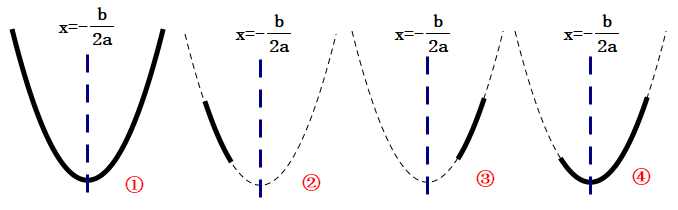
\includegraphics[scale=0.8]{figure/6-1.PNG} 
\end{enumerate}
\item 动轴或动区间
对于二次函数$y=ax^2+bx+c(a>0)$,在$m\leq x\leq n$($m,n$为参数)条件下,函数的最值需要分别讨论$m,n$与$-\dfrac{b}{2a}$的大小.
\end{enumerate}
\subsection{二次函数的应用}
\begin{enumerate}
\item 常见应用题类型按照考频从高到低可以分为:
\begin{enumerate}[(1)]
\item 经济利润问题
\item 方案选择类问题
\item 行程问题
\item 建模类问题
\item 工程问题
\end{enumerate}
\item 解应用题的关键在于审题,理解题意,尤其是一些条件范围的限制,然后再列出相应的方程、不等式、一次函数、二次函数关系式求解。其中二次函数求最值是最常见的考点,在求最值的过程中一定要注意自变量的取值范围。
\end{enumerate}
\subsection{二次函数和方程综合}
\begin{enumerate}
\item 函数$y=a_1x+b_1$和二次函数$y=a_2x^2+b_2x+c$的交点
\begin{enumerate}[(1)]

\begin{shaded}
\item 交点求解,联立方程组$ \begin{cases}
y=a_1x+b_1\\
y=a_2x^2+b_2x+c
\end{cases}$,并代入求解.
\item 交点个数,联立方程组$ \begin{cases}
y=a_1x+b_1\\
y=a_2x^2+b_2x+c
\end{cases}$,消元得到一元二次方程,看判别式$(\Delta)$.
\item 交点关系,联立方程组$ \begin{cases}
y=a_1x+b_1\\
y=a_2x^2+b_2x+c
\end{cases}$,看判别式$(\Delta)$,再利用韦达定理.
\end{shaded}

\end{enumerate}
\item 一元二次方程$a_1x+b_1=a_2x^2+b_2x+c$的解也可以看成函数$y=a_1x+b_1$和二次函数$y=a_2x^2+b_2x+c$的交点的横坐标.
\item 二次函数与一元二次方程的关系(二次函数与$x$轴的交点情况):

\begin{shaded}
一元二次方程$ax^2+bx+c=0$是二次函数$y=ax^2+bx+c$当函数值$y=0$时的特殊情况.

图象与$x$轴的交点个数:

\ding{192}当$\Delta=b^2-4ac>0$时,图象与$x$轴交于两点$A(x_1,y_1),B(x_2,y_2)(x_1\neq x_2)$,其中的$x_1,x_2$是一元二次方程$ax^2+bx+c=0(a\neq 0)$的两根.这两点间的距离$AB=\abs{x_2-x_1}=\dfrac{\sqrt{b^2-4ac}}{\abs{a}}$.

\ding{193}当$\Delta=0$时,图象与$x$轴只有一个交点;

\ding{194}当$\Delta<0$时,图象与$x$轴没有交点.此时:

~~~~~$1'$~~当$a>0$时,图象落在$x$轴的上方,无论$x$为任何实数,都有$y>0$;

~~~~~$2'$~~当$a<0$时,图象落在$x$轴的下方,无论$x$为任何实数,都有$y<0$.
\end{shaded}
\item 抛物线$y=ax^2+bx+c$的图象与$y$轴一定相交,交点坐标为$(0,c)$;
\item 二次函数常用解题方法总结:
\begin{enumerate}[(1)]

\begin{shaded}
\item 求二次函数的图象与$x$轴的交点坐标,需转化为一元二次方程;
\item 求二次函数的最大(小)值需要利用配方法将二次函数由一般式转化为顶点式;
\item 根据图象的位置判断二次函数$y=ax^2+bx+c$中$a,b,c$的符号,或由二次函数中$a,b,c$的符号判断图象的位置,要数形结合;
\item 二次函数的图象关于对称轴对称,可利用这一性质,求和已知一点对称的点坐标,或已知与$x$轴的一个交点坐标,可由对称性求出另一个交点坐标;
\item 与二次函数有关的还有二次三项式,二次三项式$ax^2+bx+c(a\neq 0)$本身就是所含字母$x$的二次函数;
\end{shaded}

下面以$a>0$时为例,揭示二次函数、二次三项式和一元二次方程之间的内在联系:
\begin{table}[ht]
\centering
\begin{tabular}{|l|l|l|l|}
\hline
$\Delta >0$&\makecell{抛物线与$x$轴有两个交点}&\makecell{二次三项式的值可正、可零、可负}&\makecell{一元二次方程有两个不相等实根}\\ \hline
$\Delta =0$&\makecell{抛物线与$x$轴只有一个交点}&\makecell{二次三项式的值为非负}&\makecell{一元二次方程有两个相等实根}\\
\hline
$\Delta <0$&\makecell{抛物线与$x$轴无交点}&\makecell{二次三项式的值恒为正}&\makecell{一元二次方程无实根}\\
\hline
\end{tabular}
\end{table}
\end{enumerate}
\end{enumerate}
\subsection{二次函数的线段最值}

\centering
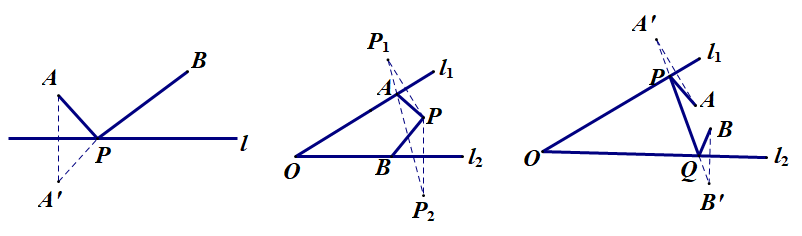
\includegraphics[scale=0.6]{figure/9-1.PNG} \\
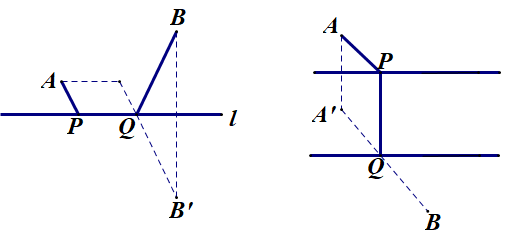
\includegraphics[scale=0.7]{figure/9-2.PNG} 

\begin{enumerate}
\item 定点在同侧,需要对称轴化为异侧;
\item 动线段端点不重合,需要平移转化到同一点.
\end{enumerate}
\subsection{二次函数和不等式综合}
\begin{enumerate}
\item 数形结合,可以通过二次函数和其它函数的图象解不等式.
\item 根的分布:一元二次方程根的分布问题,即一元二次方程的实根在什么区间内的问题,实质就是其相应二次函数的零点(图象与$x$轴的交点)问题,因此,借助于二次函数及其图象利用数形结合的方法来研究是非常有益的.
\begin{enumerate}[(1)]
\item $0$分布或$k$分布
\item 区间分布

\centering
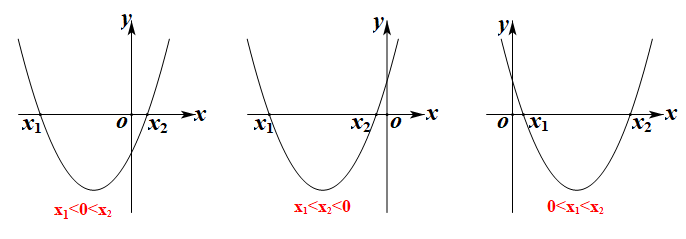
\includegraphics[scale=0.5]{figure/10-1.PNG} \\
\centering
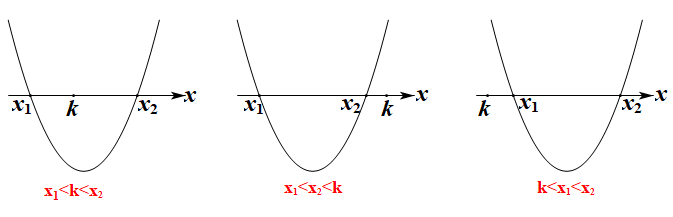
\includegraphics[scale=0.5]{figure/10-2.PNG} \\
\centering
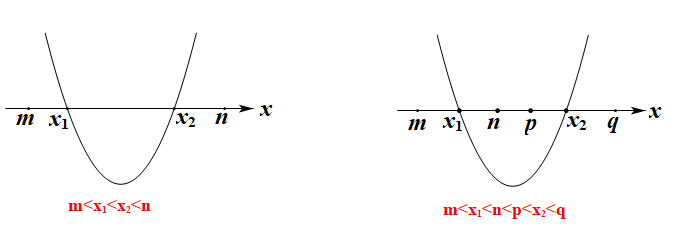
\includegraphics[scale=0.5]{figure/10-3.PNG} 

\end{enumerate}
\end{enumerate}
\subsection{二次函数的面积最值}
\begin{enumerate}
\item 铅垂法:$S=\dfrac{1}{2}\times$ 水平宽$\times$ 铅垂高.

分三步走:(1)过动点做铅垂线,交另外两个定点连成的直线与一点;(2)设出点坐标,表示线段长;(3)利用二次函数配方求最值.
\item 切线法:直线与抛物线相切,即联立解析式使$\Delta=0$.
\end{enumerate}
\section{例题分析}
\subsection{题型一:二次函数的定义}
\begin{dkyi}{}{}
   \begin{enumerate}[(1)]
   \item 在函数\ding{192}$y=\sqrt{3}x^2+\dfrac{1}{2}x+1$;\ding{193}$y=(3x+2)(4x-3)-12x^2$;\ding{194}$y=ax^2+bx+c(a,b,c\text{是常数})$;\\ \ding{195}$y=x^2+kx+20(k\text{是常数})$;\ding{196}$y=x^2+\dfrac{5}{x^2}+6$中,$y$关于$x$二次函数是\underline{~\hspace{2cm}~}
   \item 当$m=$\underline{~\hspace{2cm}~}时,$y=(m^2-4)x^{m^2-m-4}+x+3$是二次函数.
   \item 下列函数关系中,可以看作二次函数$y=ax^2+bx+c(a\neq 0)$模型的是\underline{~\hspace{2cm}~}
   \begin{enumerate}[A.]
   \item 圆的周长与半径之间的关系
   \item 在一定距离内,汽车行驶的速度与行驶的时间的关系
   \item 矩形周长一定时,矩形面积和矩形边长之间的关系
   \item 我国人口的自然增长率为$1\%$,这样我国总人口数随年份变化的关系
   \end{enumerate}
   \end{enumerate}
\end{dkyi}
\begin{jply}{}{}
   \begin{enumerate}[(1)]
   \item 下列函数:\ding{192}$y=\dfrac{1}{x^2}$;\ding{193}$y=(x-1)(x+3)$;\ding{194}$y=x^2+bx+c(b,c\text{为常数})$;\ding{195}$y=ax+x^2+3(a\text{为常数})$;\ding{196}$y=(x-1)^2-(x+1)(x-1)$,其中是二次函数的是\underline{~\hspace{2cm}~}
   \item 当$m=$\underline{~\hspace{2cm}~}时,函数$y=(m-4)x^{m^2-5m+6}+3x$是关于$x$的二次函数.
   \item 已知函数$y=(m^2+m)x^{m^2-m}+(m^2+3m+2)x+2m$是二次函数,则函数为\underline{~\hspace{2cm}~}
   \end{enumerate}
\end{jply}

\subsection{题型二:二次函数的图象与性质}
\begin{dkyi}{}{}
  \begin{enumerate}[(1)]
  \item 若二次函数$y=ax^2+bx+a^2-2(a,b\text{为常数})$图象如下左图,则$a$值\underline{~\hspace{2cm}~}.
  \item 如下右图,抛物线\ding{192}\ding{193}\ding{194}\ding{195}对应的解析式为$y=a_1x^2,y=a_2x^2,y=a_3x^2,y=a_4x^2$,将$a_1,a_2,a_3,a_4$从小到大排列为\underline{~\hspace{2cm}~}.
  \end{enumerate}
\end{dkyi}

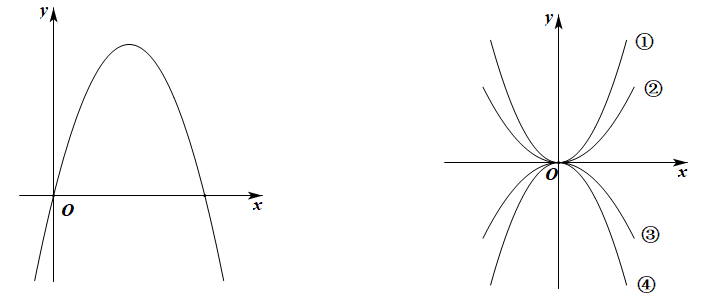
\includegraphics[scale=0.6]{figure/l-2.PNG} 
\begin{dkyi}{}{}
  \begin{enumerate}[(1)]
  \item 抛物线$y=2x^2+bx+3$的对称轴是直线$x=-2$,则$b$的值为\underline{~\hspace{1cm}~},顶点坐标为\underline{~\hspace{1cm}~}.
  \item 抛物线$y=ax^2-2ax-3a(a\neq 0)$的对称轴是直线\underline{~\hspace{1cm}~},与$x$轴的交点为\underline{~\hspace{1cm}~}和\underline{~\hspace{1cm}~}.
  \item 二次函数$y=x^2-2(k+1)x+4$的顶点在$y$轴上,则$k=$\underline{~\hspace{1cm}~},若顶点在$x$轴上,则$k=$\underline{~\hspace{1cm}~}.
  \end{enumerate}
\end{dkyi}
\begin{dkyi}{}{}
  \begin{enumerate}[(1)]
  \item 若点$A(2,y_1),B(-3,y_2),C(5,y_3)$三点在抛物线$y=x^2-4x-m$的图象上,则$y_1,y_2,y_3$的大小关系是
  \onech{$y_1>y_2>y_3$}{$y_2>y_1>y_3$}{$y_2>y_3>y_1$}{$y_3>y_2>y_1$}
  
  \item 已知二次函数$y=ax^2-4ax+c(a<0)$,当自变量$x$分别取$\sqrt{2},3,0$时,对应的值分别为$y_1,y_2,y_3$,则$y_1,y_2,y_3$的大小关系正确的是
 
  \onech{$y_3<y_2<y_1$}{$y_1<y_2<y_3$}{$y_2<y_1<y_3$}{$y_3<y_1<y_2$}
 
  \item 已知二次函数$y=-x^2-(m-1)x+1$,当$x<1$时,$y$随$x$的增大而增大,则$m$范围是\underline{~\hspace{1cm}~}.
  \end{enumerate}
\end{dkyi}
\begin{jply}{}{}
   \begin{enumerate}[(1)]
   \item 已知抛物线经过点$A(-2,7),B(6,7),C(3,-8),D(m,-8)$,则$m=$\underline{~\hspace{1cm}~}.
   \item 已知抛物线$y=x^2+2x+1$经过点$A(m,n),B(m+6,n)$,则$n=$\underline{~\hspace{1cm}~}.
   \item 已知点$A(x_1,5),B(x_2,5)$是函数$y=x^2-mx+3$上两点,则当$x=x_1+x_2$和$x=$\underline{~\hspace{1cm}~}时的函数值相等.
   \end{enumerate}
\end{jply}
\begin{jply}{}{}
   \begin{enumerate}[(1)]
   \item 已知二次函数$y=(x-3)^2+1$,下列说法:\ding{192}其图象的开口向下;\ding{193}其图象的对称轴为直线$x=3$;\ding{194}其图象顶点坐标为$(3,-1)$;\ding{195}当$x<3$时,$y$随$x$的增大而减小.则正确的有
   
   \onech{$1$个}{$2$个}{$3$个}{$4$个}
   
   \item 对于二次函数$y=x^2-2mx+3(m>0)$,有下列说法:
   
   \ding{192}如果$m=2$,则$y$有最小值$-1$;
   
   \ding{193}如果当$x\leqslant 1$时,$y$随$x$的增大而减小,则$m=1$;
   
   \ding{194}如果当$x=1$时的函数值与$x=2015$时的函数值相等,则当$x=2016$时的函数值为$3$.
   
   其中正确的是\underline{~\hspace{1cm}~}.(把你认为正确的结论的序号都填上)
   \item 在同一直角坐标系中,函数$y=mx+m$和函数$y=-mx^2+2x+2(m\text{是常数,且}m\neq 0)$的图象可能是
   \end{enumerate}
\end{jply}

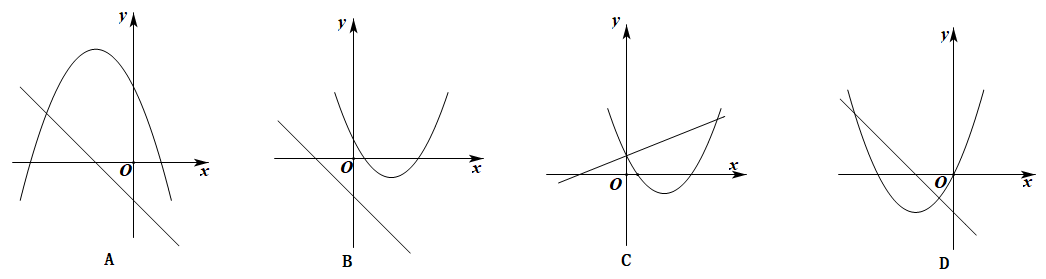
\includegraphics[scale=0.6]{figure/g-3.PNG} 
\subsection{题型三:二次函数的解析式}
\begin{dkyi}{}{}
  \begin{enumerate}[(1)]
  \item 一个二次函数图象经过$A(1,0),B(2,3),C(3,28)$三点,求二次函数解析式.
  \item 已知一个二次函数的图象经过$A(0,-1),B(1,5),C(-1,-3)$三点,求此二次函数的解析式并把二次函数转化成顶点式.
  \end{enumerate}
\end{dkyi}
\begin{dkyi}{}{}
  \begin{enumerate}[(1)]
  \item 已知二次函数过点$(0,-1)$,且顶点为$(-1,2)$,求二次函数的解析式.
  \item 已知二次函数的顶点坐标为$(2,-2)$,且其图象经过点$(3,1)$,求此二次函数的解析式,并求出该函数图象与$x$轴的交点坐标.
  \end{enumerate}
\end{dkyi}
\begin{jply}{}{}
   \begin{enumerate}[(1)]
   \item 若抛物线经过$(-3,0)$,$(1,0)$,且与$y$轴交点为$(0,4)$,求二次函数的解析式.
   \item 二次函数$y=ax^2+bx+c$对称轴为$x=2$,且经过点$(1,4),(5,0)$,求此二次函数的解析式.
   \end{enumerate}
\end{jply}
\begin{jply}{}{}
   \begin{enumerate}[(1)]
   \item 已知二次函数图象经过点$A(1,3),B(0,2),C(5,3)$,求二次函数解析式.
   \item 已知函数$y=x^2-\abs{x}-12$的图象与$x$轴交于相异两点$A,B$,另一抛物线$y=ax^2+bx+c$过$A,B$,顶点为$P$,且$\Delta APB$是等腰直角三角形,求$a,b,c$.
   \end{enumerate}
\end{jply}
\subsection{题型四:二次函数的图象综合}
\begin{dkyi}{}{}
  \begin{enumerate}[(1)]
  \item 二次函数$y=ax^2+bx+c$的图象如图$1$,则一次函数$y=(a+b)x+ac$的图象不经过
  
  \onech{第一象限}{第二象限}{第三象限}{第四象限}
  \item 二次函数$y=ax^2+bx+c$的图象如图$2$,则下列六个代数式:$ab,ac,a+b+c,a-b+c,2a+b,2a-b,b^2-4ac$中,其值为正的式子的个数是
  
  \onech{$5$个}{$4$个}{$3$个}{$2$个}
  \item 二次函数$y=ax^2+bx+c$的图象如图$3$,则$\abs{a+b+c}-\abs{a-b+c}+\abs{2a+b}-\abs{2a-b}$\underline{~\hspace{1cm}~}$0$.(填$>$、$<$或$=$).
  \end{enumerate}
\end{dkyi}

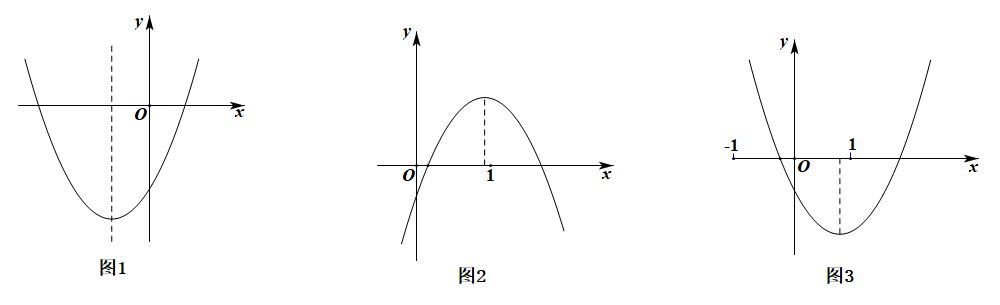
\includegraphics[scale=0.6]{figure/l-7.PNG} 
\begin{dkyi}{}{}
  \begin{enumerate}[(1)]
  \item 已知二次函数$y=ax^2+bx+c$的图象如图$1$所示,有下列结论:\ding{192}$b^2-4ac>0$;\ding{193}$abc>0$;\ding{194}$2a+b>0$;\ding{195}$9a+3b+c<0$;\ding{196}$8a+c>0$.正确的有\underline{~\hspace{1cm}~}.
  \item 如图$2$,抛物线$y=ax^2+bx+c$的图象交$x$轴于$A(x_1,0),B(2,0)$,交$y$轴正半轴于$C$,且$OA=OC$,下列结论:\ding{192}$\dfrac{a-b}{c}>0$;\ding{193}$ac=b-1$;\ding{194}$a=-\dfrac{1}{2}$;\ding{195}$2b+c=2$.其中结论正确的有\underline{~\hspace{1cm}~}.
  \end{enumerate}
\end{dkyi}

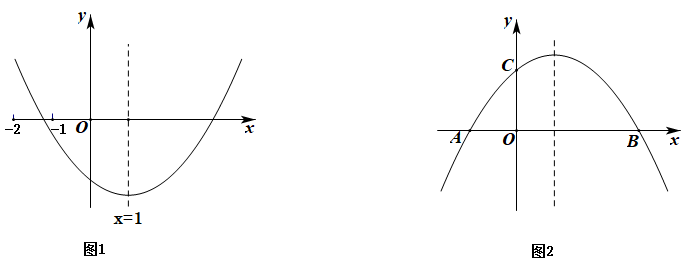
\includegraphics[scale=0.6]{figure/l-8.PNG} 
\begin{dkyi}{}{}
  \begin{enumerate}[(1)]
  \item 已知二次函数$y=ax^2+bx+c+2$的图象如图$1$所示,顶点为$(-1,0)$,下列结论:\ding{192}$abc<0$;\ding{193}$b^2-4ac=0$;\ding{194}$a>2$;\ding{195}$4a-2b+c>0$.其中正确结论的个数是\underline{~\hspace{1cm}~}.
  \item 二次函数$y=ax^2+bx+c$的图象如图$2$所示,给出下列结论::\ding{192}$2a+b>0$;\ding{193}若$-1<m<n<1$,则$m+n<-\dfrac{b}{a}$;\ding{194}$3\abs{a}+\abs{c}<2\abs{b}$;\ding{195}$b>a>c$.其中正确的结论有\underline{~\hspace{1cm}~}.
  \end{enumerate}
\end{dkyi}

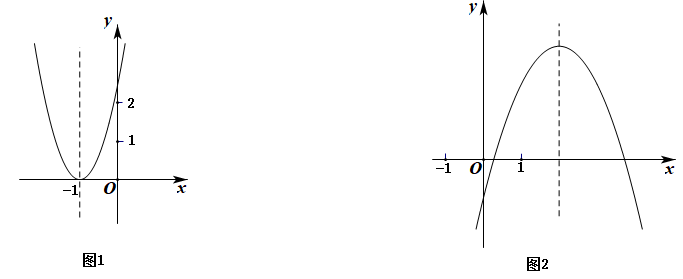
\includegraphics[scale=0.6]{figure/l-9.PNG} 
\begin{dkyi}{}{}
  \begin{enumerate}[(1)]
  \item 二次函数$y=ax^2+bx+c$的图象如图$1$,则一次函数$y=ax-\dfrac{b}{c}$的图象不经过第\underline{~\hspace{1cm}~}象限.
  \item 如图$2$,二次函数$y=ax^2+bx+c$的图象经过点$(-1,2)$和$(1,0)$,给出五个结论:\ding{192}$abc<0$;\ding{193}$2a+b>0$;\ding{194}$a+c=1$;\ding{195}$a>1$;\ding{196}$9a+6b+4c>0$.其中结论正确的是\underline{~\hspace{1cm}~}.
  \item 二次函数$y=ax^2+bx+c$的图象如图$3$,小丹观察得出了下面五条信息:\ding{192}$c<0$;\ding{193}$abc>0$;\ding{194}$a-b+c>0$;\ding{195}$2a-3b=0$;\ding{196}$c-4b>0$.其中结论正确的是\underline{~\hspace{1cm}~}.
  \end{enumerate}
\end{dkyi}

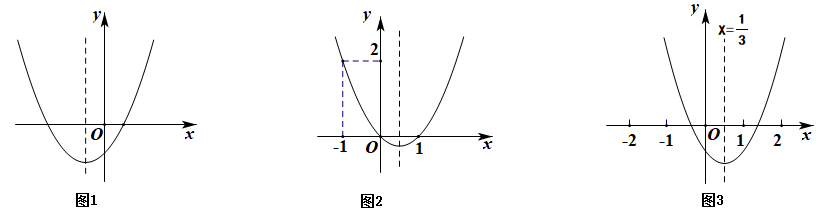
\includegraphics[scale=0.6]{figure/l-10.PNG} 
\begin{jply}{}{}
    \begin{enumerate}[(1)]
  \item 如图$1$,二次函数$y=ax^2+bx+c$的图象经过点$(-1,2)$,下列结论:\ding{192}$4a-2b+c<0$;\ding{193}$2a-b<0$;\ding{194}$b<-2$;\ding{195}$(a+c)^2<b^2$.其中正确的结论有\underline{~\hspace{1cm}~}(填序号)
  \item 如图$2$,已知二次函数$y=ax^2+bx+c$的图象经过点$(1,2)$,下列结论:\ding{192}$2a+b<0$;\ding{193}$abc<0$;\ding{194}$a+c<-1$;\ding{195}$b^2+8a<4ac$.其中结论正确的是\underline{~\hspace{1cm}~}(填序号).
  \item 二次函数$y=ax^2+bx+c(a\neq 0)$的图象如图$3$,有下列五个结论:\ding{192}$abc<0$;\ding{193}$b<a+c$;\ding{194}$4a+2b+c>0$;\ding{195}$b^2-4ac>0$;\ding{196}$a+b>m(am+b)$($m\neq 1$的实数).其中结论正确的是\underline{~\hspace{1cm}~}(填序号).
  \end{enumerate}
\end{jply}

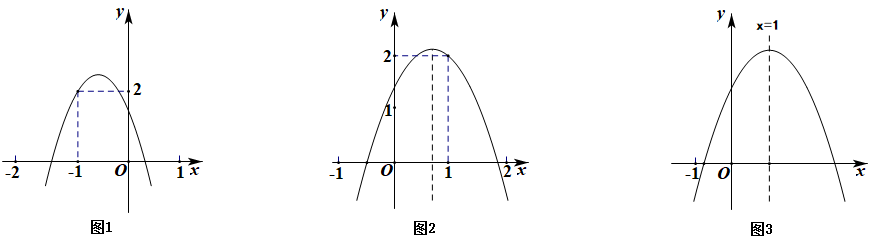
\includegraphics[scale=0.6]{figure/g-6.PNG} 
\begin{jply}{}{}
    \begin{enumerate}[(1)]
  \item 已知二次函数$y=ax^2+bx+c(a\neq 0)$的图象如图$1$所示,它与$x$轴两个交点分别为$(-1,0),(3,0)$,对于下列命题:\ding{192}$b-2a=0$;\ding{193}$abc<0$;\ding{194}$-a-\dfrac{1}{2}b+c<0$;\ding{195}$8a+c>0$.其中正确的结论有\underline{~\hspace{1cm}~}(填序号)
  \item 如图$2$,抛物线$y=ax^2+bx+c(a\neq 0)$的对称轴是$x=-1$,且过点$(\dfrac{1}{2},0)$,有下列结论:\ding{192}$abc>0$;\ding{193}$a-2b+4c=0$;\ding{194}$25a-10b+4c=0$;\ding{195}$3b+2c>0$.其中结论正确的是\underline{~\hspace{1cm}~}(填序号).
  \item 如图$3$,二次函数$y=ax^2+bx+c(a\neq 0)$的图象与$x$轴交于点$A(-1,0)$,对称轴为直线$x=1$,与$y$轴的交点$B$在$(0,2)$和$(0,3)$之间(包括这两点),有下列结论:\ding{192}当$x>3$时,$y<0$;\ding{193}$3a+b<0$;\ding{194}$-1\leq a\leq -\dfrac{2}{3}$;\ding{195}$4ac-b^2>8a$.其中结论正确的是\underline{~\hspace{1cm}~}(填序号).
  \end{enumerate}
\end{jply}

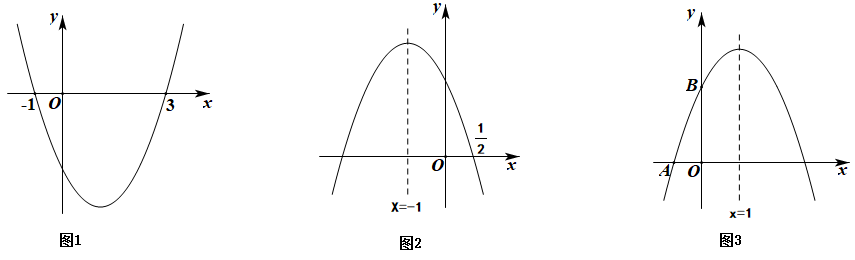
\includegraphics[scale=0.6]{figure/g-7.PNG} 
\subsection{题型五:二次函数的图象变换}
\begin{dkyi}{}{}
  \begin{enumerate}[(1)]
  \item 二次函数$y=-2x^2+4x+1$的图象如何移动就得到$y=-2x^2$的图象
  
  \twoch{向左移动$1$个单位,向上移动$3$个单位}{向右移动$1$个单位,向上移动$3$个单位}{向左移动$1$个单位,向下移动$3$个单位}{向右移动$1$个单位,向下移动$3$个单位}
  \item 一抛物线向右平移$3$个单位,再向下平移$2$个单位后得到抛物线$y=-2x^2+4x$,则平移前抛物线的解析式为\underline{~\hspace{1cm}~}.
  \item 如果抛物线$y=-2x^2+8$向右平移$a$个单位后,恰好过点$(3,6)$,那么$a$值为\underline{~\hspace{1cm}~}.
  \end{enumerate}
\end{dkyi}
\begin{dkyi}{}{}
已知二次函数$y=x^2-2x-1$,求:

$(1)$与此二次函数关于$x$轴对称的二次函数解析式为\underline{~\hspace{1cm}~}.

$(2)$与此二次函数关于$y$轴对称的二次函数解析式为\underline{~\hspace{1cm}~}.

$(3)$与此二次函数关于原点对称的二次函数解析式为\underline{~\hspace{1cm}~}.
\end{dkyi}
\begin{dkyi}{}{}
 已知二次函数$y=ax^2+4ax+4a-1$的图象是$C_1$.
 
 $(1)$求$C_1$关于点$R(1,0)$中心对称的图象$C_2$的解析式;
 
 $(2)$设曲线$C_1,C_2$与$y$轴的交点分别为$A,B$,当$\abs{AB}=18$时,求$a$的值.
\end{dkyi}
\begin{jply}{}{}
   \begin{enumerate}[(1)]
   \item 如图,已知抛物线$C_0$的解析式为$y=x^2-2x$,则抛物线$C_0$的顶点坐标\underline{~\hspace{1cm}~};将抛物线$C_0$每次向右平移$2$个单位,平移$n$次,依次得到抛物线$C_1,C_2,\cdots,C_n$($n$为正整数),则抛物线$C_n$的解析式为\underline{~\hspace{1cm}~}.
   \item 如图,把抛物线$y=\dfrac{1}{2}x^2$平移得到抛物线$m$,抛物线$m$经过点$A(-6,0)$和原点$O(0,0)$,它的顶点为$P$,它的对称轴与抛物线$y=\dfrac{1}{2}x^2$交于点$Q$,则图中阴影部分的面积为\underline{~\hspace{1cm}~}.
   \end{enumerate}
\end{jply}
\begin{jply}{}{}
   已知关于$x$的一元二次方程$2x^2+4x+k-1=0$有实数根,$k$为正整数.
   
   $(1)$求$k$的值;
   
   $(2)$当此方程有两个非零的整数根时,将关于$x$的二次函数$y=2x^2+4x+k-1$的图象向下平移$8$个单位,求平移后的图象的解析式;
   
   $(3)$在$(2)$的条件下,将平移后的二次函数的图象在$x$轴下方的部分沿$x$轴翻折,图象的其余部分保持不变,得到一个新的图象,请结合这个新的图象回答:当直线$y=\dfrac{1}{2}x+b(b<k)$与此图象有两个公共点时,$b$的取值范围.
\end{jply}
\subsection{题型六:二次函数在闭区间上的最值}
\begin{dkyi}{}{}
  分别求出在下列条件下,函数$y=-2x^2+3x+1$的最值.
  
  $(1)$ $x$取任意实数;$(2)$当$-2\leqslant x\leqslant 0$时;$(3)$当$1\leqslant x\leqslant 3$时;$(4)$当$-1\leqslant x\leqslant 2$时.
\end{dkyi}
\begin{jply}{}{}
   \begin{enumerate}[(1)]
   \item 求函数$y=2x^2-x+1$的最小值;
   \item 若$1\leqslant x\leqslant 2$,求$y=2x^2-x+1$的最大值、最小值;
   \item 若$0\leqslant x\leqslant 1$,求$y=2x^2-x+1$的最大值、最小值;
   \item 若$-2\leqslant x\leqslant 0$,求$y=2x^2-x+1$的最大值、最小值.
   \end{enumerate}
\end{jply}
\begin{jply}{}{}
   试求$y=(x+1)(x+2)(x+3)(x+4)+5$在$-3\leqslant x\leqslant 3$的最值.
\end{jply}
\begin{dkyi}{}{}
  已知函数$y=x^2-2x+2$在$t\leqslant x\leqslant t+1$范围内的最小值为$s$,写出函数$s$关于$t$的函数解析式.
\end{dkyi}
\begin{dkyi}{}{}
  已知函数$y=-9x^2-6ax-a^2+2a$在区间$-\dfrac{1}{3}\leqslant x\leqslant \dfrac{1}{3}$有最大值$-3$,求实数$a$的值.
\end{dkyi}
\begin{jply}{}{}
   已知函数$y=-x^2+2ax+1-a$在$0\leqslant x\leqslant 1$上有最大值$2$,求$a$的值.
\end{jply}
\begin{jply}{}{}
   设$y=x^2+ax+3-a$,当$-2\leqslant x\leqslant 2$时,$y$的最小值不小于$0$,求实数$a$范围.
\end{jply}
\begin{jply}{}{}
   若函数$y=-\dfrac{1}{2}x^2+\dfrac{13}{2}$在区间$a\leq x\leq b(b>a)$上的最小值为$2a$,最大值为$2b$,求$a,b$的值.
\end{jply}
\subsection{题型七:二次函数应用}
\begin{dkyi}{}{}
某超市销售某种玩具,进货价为$20$元,根据市场调查:在一段时间内,销售单价是$30$元时,销售量是$400$件,而销售单价每上涨$1$元,就会少出售$10$件玩具,超市要完成不少于$300$件的销售任务,当销售单价定为多少元时,可获得最大利润,最大利润是多少元?
\end{dkyi}
\begin{dkyi}{}{}
 某果园有$100$棵橙子树,平均每棵树结$600$个橙子,现准备多种一些橙子树以提高果园产量,但是如果多种树,那么树之间的距离和每一棵树所接受的阳光就会减少.根据经验估计,每多种一棵树,平均每棵树就会少结$5$个橙子,假设果园多种了$x$棵橙子树.
 
 $(1)$直接写出平均每棵树结的橙子个数$y$(个)与$x$之间的关系;
 
 $(2)$果园多种多少棵橙子树时,可使橙子的总产量最大?最大为多少个?
\end{dkyi}
\begin{jply}{}{}
 九$(1)$班数学兴趣小组经过市场调查,整理出某种商品在第$x(1\leq x\leq 90)$天的售价与销量的相关信息如下表:
 已知该商品的进价为每件$30$元,设销售该商品的每天利润为$y$元.
  

 \begin{tabular}{|p{3cm} |p{4cm}|p{4cm}|}
 \hline
 时间$x$(天)&$1\leq x<50$&$50\leq x\leq 90$\\ \hline
 售价(元/件)&$x+40$&$90$\\ \hline
 每天销量(件)& \multicolumn{2}{c|}{$200-2x$}\\ \hline
 \end{tabular}

 
 $(1)$求出$y$与$x$的函数关系式;
 
 $(2)$问销售该商品第几天时,当天销售利润最大,最大利润是多少?
 
 $(3)$该商品在销售过程中,共有多少天每天销售利润不低于$4800$元?请直接写出结果.
\end{jply}
\begin{jply}{}{}
某集团公司试销一种成本为每件$60$元的节能产品,规定试销期间销售单价不低于成本单价,且获利不将高于$40\%$.经试销发现,销售量$y$(万件)与销售单价$x$(元)之间的函数图象如图.

  $(1)$求$y$与$x$之间的函数关系式,并写出自变量$x$的取值范围;
 
 $(2)$设该集团公司销售这种节能产品获得利润为$W$(万元),试求出利润$W$(万元)与销售单价$x$(元)之间的函数关系式;并求出当销售单价定为多少元时,公司可获得最大利润,最大利润是多少万元?
 
 $(3)$该公司决定每销售一件产品,就抽出$5$元钱捐给希望工程,若除去捐款后,所获利润不低于$450$万元,请你确定此时销售单价的范围.
 \end{jply}
\subsection{题型八:二次函数和方程综合}
\begin{dkyi}{}{}
  \begin{enumerate}[(1)]
  \item 抛物线$y=x^2+5x+a^2$与一次函数$y=ax+2a-1$有交点,则$a$的范围\underline{~\hspace{1cm}~}.
  \item 已知函数$y=mx^2-3x+2$($m$是常数),若一次函数$y=x+1$的图象与该函数的图象恰好只有一个交点,则交点坐标为\underline{~\hspace{1cm}~}.
  \end{enumerate}
\end{dkyi}
\begin{dkyi}{}{}
  \begin{enumerate}[(1)]
  \item 二次函数$y=ax^2+bx+c$的图象如图所示,则关于$x$的方程$ax^2+bx+c+3=0$的根的情况是
  
  \twoch{有两个相等的实数根}{无实数根}{有两个同号不相等实数根}{有两个异号实数根}
  \item 若方程$\abs{x^2-4x+3}=m$有两个相异的实数解,则$m$范围是\underline{~\hspace{1cm}~}.
  \end{enumerate}
\end{dkyi}
\begin{jply}{}{}
   \begin{enumerate}[(1)]
   \item 二次函数$y=x^2+kx+k-1$的图象与$x$轴的交点个数\underline{~\hspace{1cm}~}.
   \item 给出定义:设一条直线与一条抛物线只有一个公共点,且这条直线与这条抛物线的对称轴不平行,就称直线与抛物线相切,这条直线是这条抛物线的切线,有下列命题:
   
   \ding{192}直线$y=0$是抛物线$y=\dfrac{1}{4}x^2$的切线;
   
   \ding{193}直线$x=-2$与抛物线$y=\dfrac{1}{4}x^2$相切于点$(-2,1)$;
   
   \ding{194}直线$y=x+b$与抛物线$y=\dfrac{1}{4}x^2$相切,则相切于点$(2,1)$;
   
   \ding{195}直线$y=kx-2$与抛物线$y=\dfrac{1}{4}x^2$相切,则$k=\pm \sqrt{2}$.
   
   其中正确的命题有\underline{~\hspace{1cm}~}.
   \item 若方程$\abs{x^2-5x}=a$有四个不相等实根,则$a$的取值范围是\underline{~\hspace{1cm}~}.
   \end{enumerate}
\end{jply}
\begin{dkyi}{}{}
 已知二次函数$y=x^2-x+c$.
 
 $(1)$若点$A(-1,n),B(2,2n-1)$在二次函数$y=x^2-x+c$的图象上,求此二次函数的最小值;
 
 $(2)$若$D(2,y_1),E(x_2,2)$关于坐标原点成中心对称,试判断直线$DE$与抛物线$y=x^2-x+c+\dfrac{3}{8}$的交点个数,并说明理由.
\end{dkyi}
\begin{jply}{}{}
  已知二次函数$y_1=x^2-2x-3$及一次函数$y_2=x+m$.
  
  $(1)$求该二次函数图象的顶点坐标以及它与$x$轴的交点坐标;
  
  $(2)$将该二次函数图象在$x$轴下方的部分沿$x$轴翻折到$x$轴上方,图象的其余部分不变,得到一个新图象,请你在图中画出这个新图象,并求出新图象与直线$y_2=x+m$有三个不同公共点时$m$的值.
\end{jply}

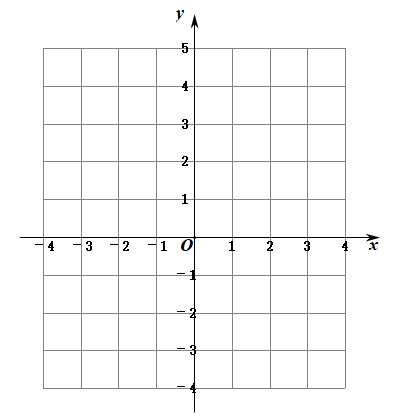
\includegraphics[scale=0.6]{figure/g-18.PNG} 
\begin{jply}{}{}
   \begin{enumerate}[(1)]
   \item 抛物线$y=x^2+\sqrt{m}x+m^2$与$x$轴两交点间距离的最大值为\underline{~\hspace{1cm}~}.
   \item 设二次函数$y=ax^2+bx+c$经过点$A(0,2),B(1,-1)$,且其图象在$x$轴上所截得的线段长为$2\sqrt{2}$,求这个二次函数的解析式.
   \end{enumerate}
\end{jply}
\begin{jply}{}{}
  已知:$y$关于$x$的函数$y=(k-1)x^2-2kx+k+2$的图象与$x$轴有交点.
  
  $(1)$求$k$的取值范围;
  
  $(2)$若$x_1,x_2$是函数图象与$x$轴两个交点的横坐标$(x_1\neq x_2)$,且满足$(k-1)x^2_1+2kx_2+k+2=4x_1x_2$.
  
  \ding{192}求$k$的值;\ding{193}当$k\leqslant x\leqslant k+2$时,求$y$的最大值与最小值.
\end{jply}
\begin{jply}{}{}
  在平面直角坐标系$xOy$中,抛物线$y=ax^2+bx+c$过点$(2,2)$,且当$x=0$时,$y$取得最小值$1$.
  
  $(1)$求此抛物线的解析式;
  
  $(2)$已知点$C(1,3)$,试探索是否存在满足下列条件的直线$l$:\ding{192}直线$l$过点$C(1,3)$;\ding{193}直线$l$交抛物线于$E,F$两点且$C$点恰好是线段$EF$的中点.若存在,请求出直线$l$的函数解析式;若不存在,请说明理由.
\end{jply}
\begin{jply}{}{}
   已知:抛物线与$x$轴交于$A(-2,0),B(4,0)$,与$y$轴交于$C(0,4)$.
   
   $(1)$求抛物线顶点$D$的坐标;
   
   $(2)$设直线$CD$交$x$轴于点$E$,过点$B$作$x$轴的垂线,交直线$CD$于点$F$,将抛物线沿其对称轴上下平移,使抛物线与线段$EF$总有公共点.试探究:抛物线向上最多可以平移多少个单位长度,向下最多可以平移多少个单位长度?
\end{jply}
\subsection{题型九:二次函数和不等式综合}
\begin{dkyi}{}{}
已知二次函数$y=x^2+bx+c$的图象如图所示,它与$x$轴的一个交点的坐标为$(-1,0)$,与$y$轴的交点坐标为$(0,-3)$.

$(1)$求二次函数的解析式,并求图象与$x$轴的另一个交点的坐标;

$(2)$根据图象回答:当$x$取何值时,$-3<y<0$.
\end{dkyi}

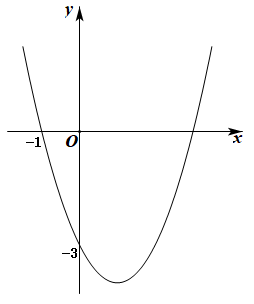
\includegraphics[scale=0.6]{figure/l-22.PNG} 
\begin{dkyi}{}{}
  \begin{enumerate}[(1)]
  \item 已知关于$x$的方程$x^2+(m-5)x+m-2=0$有实根,且方程的两根都大于$0$,则实数$m$的取值范围是\underline{~\hspace{1cm}~}.
  \item 已知方程$ax^2+(a+2)x+9a=0$的两个实根$x_1$和$x_2$,且$x_1<1<x_2$,求实数$a$取值范围.
  \end{enumerate}
\end{dkyi}
\begin{jply}{}{}
   \begin{enumerate}[(1)]
   \item 方程$x^2-11x+(30+a)=0$有两实根,两根都大于$5$,则实数$a$范围\underline{~\hspace{1cm}~}.
   \item 方程$7x^2-(p+13)x+p^2-p-2=0$的两根$\alpha,\beta$满足$0<\alpha<1<\beta<2$,求实数$p$范围.
   \end{enumerate}
\end{jply}
\begin{jply}{}{}
   \begin{enumerate}[(1)]
   \item 已知关于$x$的方程$x^2-(2-a)x+5-a=0$的一个根大于$0$而小于$2$,另一个根大于$4$而小于$6$,则实数$a$的取值范围是\underline{~\hspace{1cm}~}.
   \item 若关于$x$的方程$4x^2-2mx+n=0$的解都位于$0<x<1$的范围中,求正整数$m,n$的值.
   \end{enumerate}
\end{jply}
\subsection{题型十:二次函数的线段最值}
\begin{dkyi}{}{}
  已知抛物线$y=ax^2+bx+1$经过点$A(1,3)$和点$B(2,1)$.
  
  $(1)$求此抛物线解析式;
  
  $(2)$点$C,D$分别是$x$轴和$y$轴上的动点,求四边形$ABCD$周长的最小值.
\end{dkyi}
\begin{dkyi}{}{}
  如图,已知抛物线$y=\dfrac{k}{8}(x+2)(x-4)(k\text{为常数,且}k>0)$与$x$轴从左至右依次交于$A,B$两点,与$y$轴交于点$C$,经过点$B$的直线$y=-\frac{\sqrt{3}}{3}x+b$与抛物线的另一个交点为$D$.
  
  $(1)$若点$D$的横坐标为$-5$,求抛物线的函数表达式;
  
  $(2)$在$(1)$的条件下,设$F$为线段$BD$上一点(不含端点),连接$AF$,一动点$M$从点$A$出发,沿线段$AF$以每秒$1$个单位的速度运动到$F$,再沿线段$FD$以每秒$2$个单位的速度运动到$D$后停止.当点$F$的坐标是多少时,点$M$在整个运动过程中用时最少?
\end{dkyi}

\centering
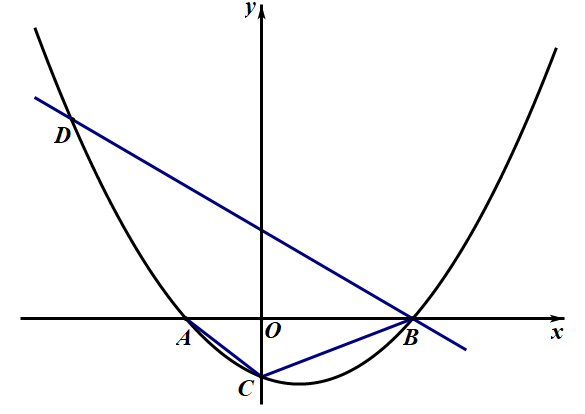
\includegraphics[scale=0.4]{figure/l-25-1.PNG} 
\begin{dkyi}{}{}
  已知抛物线$y=ax^2+bx+1$经过点$A(1,3)$和点$B(2,1)$.
  
  $(1)$求此抛物线解析式;
  
  $(2)$点$C,D$分别是$x$轴和$y$轴上的动点,求四边形$ABCD$周长的最小值;
  
  $(3)$过点$B$作$x$轴的垂线,垂足为$E$点,点$P$从抛物线的顶点出发,先沿抛物线的对称轴到达$F$点,再沿$FE$到达$E$点,若$P$点在对称轴上的运动速度是它在直线$FE$上运动速度的$\sqrt{2}$倍,试确定点$F$的位置,使得点$P$按照上述要求到达$E$点所用的时间最短.(要求:简述确定$F$点位置的方法,但不要求证明)
\end{dkyi}

\begin{dkyi}{}{}
 如图,已知抛物线$y=ax^2-4x+c$经过点$A(0,-6)$和$B(3,-9)$.
 
 $(1)$求出抛物线的解析式;
 
 $(2)$点$P(m,n)$与点$Q$均在抛物线上(其中$m>0$),且这两点关于抛物线对称轴对称,求$m$的值及点$Q$的坐标;
 
 $(3)$在满足$(2)$的情况下,在抛物线的对称轴上寻找一点$M$,使得$\Delta QMA$的周长最小.
\end{dkyi}

\raggedleft
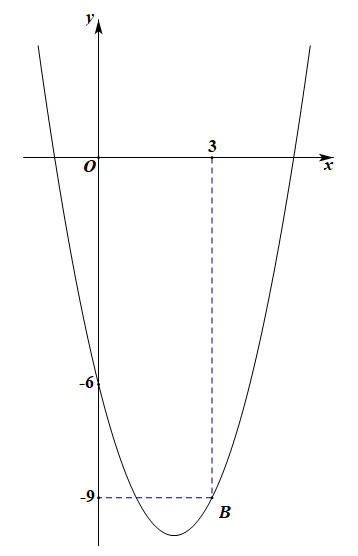
\includegraphics[scale=0.5]{figure/l-27.PNG} 
\begin{jply}{}{}
 如图,已知二次函数$y=-\dfrac{1}{2}x^2+bx+c(c<0)$的图象与$x$轴的正半轴相交于点$A,B$,与$y$轴相交于点$C$,且$OC^2=OA\bm\cdot OB$.
 
 $(1)$求$c$的值;
 
 $(2)$若$\Delta ABC$的面积为$3$,求该二次函数的解析式;
 
 $(3)$设$D$是$(2)$中所确定的二次函数图象的顶点,试问在直线$AC$是否存在一点$P$使$\Delta PBD$的周长最小?若存在,求出点$P$的坐标;若不存在,请说明理由.
\end{jply}

\raggedleft
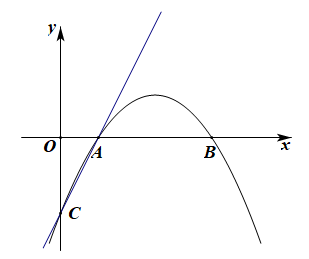
\includegraphics[scale=0.6]{figure/g-25.PNG} 
\begin{jply}{}{}
  如图,在平面直角坐标系中,$Rt\Delta AOB$的顶点坐标分别为$A(-2,0),O(0,0),B(0,4)$,把$\Delta AOB$绕点$O$按顺时针方向旋转$90^\circ$,得到$\Delta COD$.
  
  $(1)$求$C,D$两点的坐标;
  
  $(2)$求经过$A,B,D$三点的抛物线的解析式;
  
  $(3)$在$(2)$中的抛物线的对称轴上取得两点$E,F$(点$E$在点$F$的上方),且$EF=1$,如图使四边形$ACEF$的周长最小,求出$E,F$两点的坐标.
\end{jply}

\centering
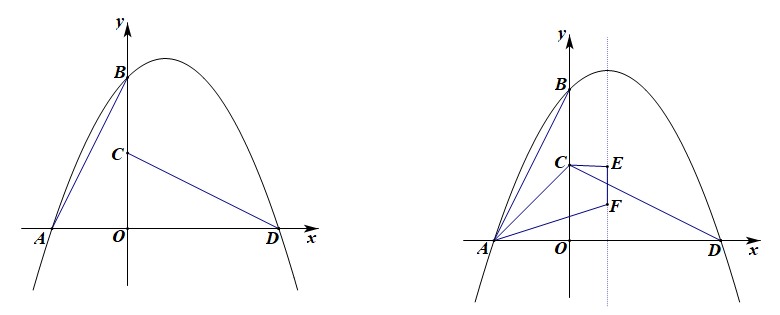
\includegraphics[scale=0.6]{figure/g-26.PNG} 
\begin{jply}{}{}
 如图,抛物线的顶点$A$的坐标$(0,2)$,对称轴为$y$轴,且经过点$(-4,4)$.
 
 $(1)$求抛物线的表达式;
 
 $(2)$若点$B$的坐标为$(0,4)$,$P$为抛物线上一点(如图),过点$P$作$PQ\perp x$轴于点$Q$,连接$PB$.求证:$PQ=PB$.
 
 $(3)$若点$C(-2,4)$,利用$(2)$的结论,判断抛物线上是否存在一点$K$,使$\Delta KBC$的周长最小?若存在,求出这个最小值,并求此时点$K$的坐标;若不存在,请说明理由.
\end{jply}

\raggedleft
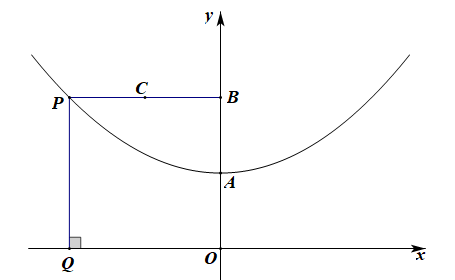
\includegraphics[scale=0.6]{figure/g-27.PNG} 

\begin{jply}{}{}
 如图,已知在平面直角坐标系$xOy$中,直角梯形$OABC$的边$OA$在$y$轴的正半轴上,$OC$在$x$轴的正半轴上,$OA=AB=2$,$OC=3$,过点$B$作$BD\perp BC$,交$OA$于点$D$,将$\angle DBC$绕点$B$按顺时针方向旋转,角的两边分别交$y$轴的正半轴、$x$轴的正半轴于点$E$和$F$.
 
 $(1)$求经过$A,B,C$三点的抛物线的解析式;
 
 $(2)$当$BE$经过$(1)$中抛物线的顶点时,求$CF$的长;
 
 $(3)$在抛物线的对称轴上取两点$P,Q$(点$Q$在点$P$的上方),且$PQ=1$,要使四边形$BCPQ$的周长最小,求出$P,Q$两点的坐标.
\end{jply}

\centering
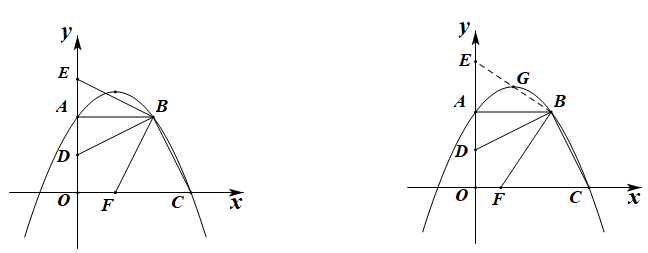
\includegraphics[scale=0.6]{figure/g-28.PNG} 
\subsection{题型十一:二次函数的面积最值}
\begin{dkyi}{}{}
  如图,已知抛物线经过点$A(-1,0),B(3,0),C(0,3)$三点.
  
  $(1)$求抛物线的解析式;
  
  $(2)$点$M$是线段$BC$上的点(不与$B,C$重合),过$M$作$MN//y$轴交抛物线于$N$,若点$M$的横坐标为$m$,请用$m$的代数式表示$MN$的长.
  
  $(3)$在$(2)$的条件下,连接$NB,NC$,是否存在$m$,使$\Delta BNC$的面积最大?若存在,求$m$的值;若不存在,说明理由.
\end{dkyi}
\raggedleft
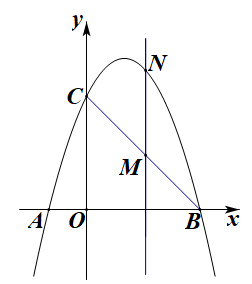
\includegraphics[scale=0.6]{figure/l-28.PNG} 
\begin{dkyi}{}{}
   已知抛物线$y=ax^2+bx+c$与$x$轴交于$A,B$两点,交$y$轴于$C$点,已知抛物线的对称轴为$x=1$,点$B(3,0)$,点$C(0,-3)$,$D$为抛物线的顶点.
   
  $(1)$求抛物线的解析式;
  
  $(2)$在$x$轴下方且在抛物线上有一动点$F$,求四边形$OBFC$的面积最大值.
\end{dkyi}

\centering
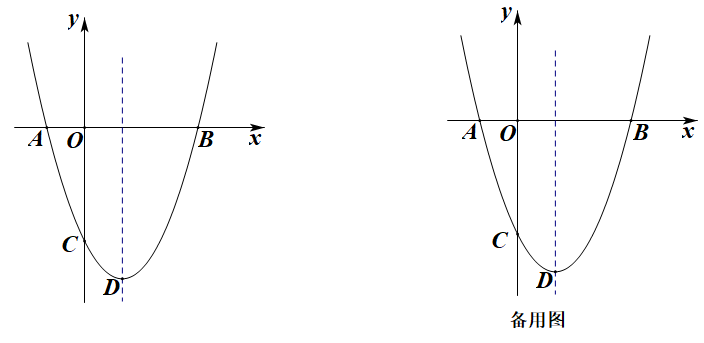
\includegraphics[scale=0.6]{figure/l-29.PNG} 
\begin{jply}{}{}
如图,在直角坐标系中有一直角三角形$AOB$,$O$为坐标原点,$OB=6,\tan \angle ABO=\dfrac{1}{3}$,将此三角形绕原点$O$逆时针旋转$90^\circ$,得到$\Delta DOC$,抛物线$y=ax^2+bx+c$经过点$A,B,C$.
 
 $(1)$ 求抛物线的解析式;
 
$(2)$若点$P$是第二象限内抛物线上的动点,其横坐标为$t$,是否存在一点$P$,使$\Delta PCD$得面积最大?若存在,求出$\Delta PCD$的面积的最大值;若不存在,请说明理由.
\end{jply}

\centering
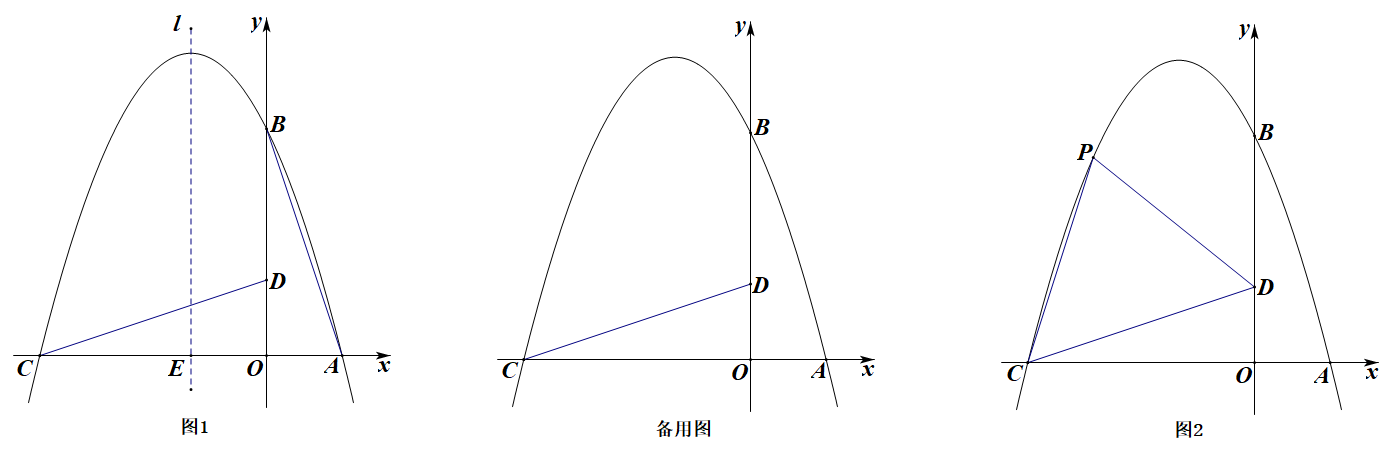
\includegraphics[scale=0.45]{figure/g-29.PNG} 
\begin{jply}{}{}
  如图,抛物线$y=ax^2+3ax+c(a>0)$与$y$轴交于$C$点,与$x$轴交于$A,B$两点,$A$点在$B$点左侧,点$B$的坐标为$(1,0),OC=3BD$.
  
  $(1)$求抛物线的解析式;
  
  $(2)$若点$D$是线段$AC$下方抛物线上的动点,求四边形$ABCD$面积的最大值.
\end{jply}

\centering
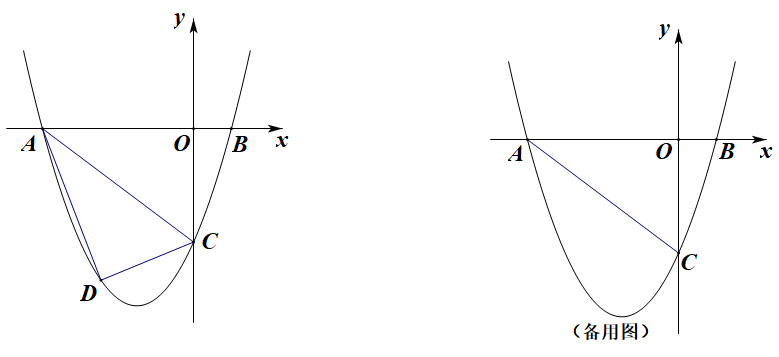
\includegraphics[scale=0.6]{figure/g-30.PNG} 
















\end{document}
